\documentclass[10pt, a4paper, twocolumn]{article} 
% PREAMBLE
%%%%%%%%%%%%%%%%%%%%%%%%%%%%%%%%%%%%%%%%%
% Wenneker Article
% Structure Specification File
% Version 1.0 (28/2/17)
%
% This file originates from:
% http://www.LaTeXTemplates.com
%
% Authors:
% Frits Wenneker
% Vel (vel@LaTeXTemplates.com)
%
% License:
% CC BY-NC-SA 3.0 (http://creativecommons.org/licenses/by-nc-sa/3.0/)
%
%%%%%%%%%%%%%%%%%%%%%%%%%%%%%%%%%%%%%%%%%

%----------------------------------------------------------------------------------------
%	PACKAGES AND OTHER DOCUMENT CONFIGURATIONS
%----------------------------------------------------------------------------------------

\usepackage[english]{babel} % English language hyphenation

\usepackage{microtype} % Better typography

\usepackage{amsmath,amsfonts,amsthm} % Math packages for equations

\usepackage[svgnames]{xcolor} % Enabling colors by their 'svgnames'

\usepackage[hang, small, labelfont=bf, up, textfont=it]{caption} % Custom captions under/above tables and figures

\usepackage{booktabs} % Horizontal rules in tables

\usepackage{lastpage} % Used to determine the number of pages in the document (for "Page X of Total")
\usepackage{amssymb}

\usepackage{graphicx} % Required for adding images

\usepackage{enumitem} % Required for customising lists
\setlist{noitemsep} % Remove spacing between bullet/numbered list elements

\usepackage{sectsty} % Enables custom section titles
\allsectionsfont{\usefont{OT1}{phv}{b}{n}} % Change the font of all section commands (Helvetica)

%----------------------------------------------------------------------------------------
%	MARGINS AND SPACING
%----------------------------------------------------------------------------------------

\usepackage{geometry} % Required for adjusting page dimensions

\geometry{
	top=1cm, % Top margin
	bottom=1.5cm, % Bottom margin
	left=2cm, % Left margin
	right=2cm, % Right margin
	includehead, % Include space for a header
	includefoot, % Include space for a footer
	%showframe, % Uncomment to show how the type block is set on the page
}

\setlength{\columnsep}{7mm} % Column separation width

%----------------------------------------------------------------------------------------
%	FONTS
%----------------------------------------------------------------------------------------

\usepackage[T1]{fontenc} % Output font encoding for international characters
\usepackage[utf8]{inputenc} % Required for inputting international characters

\usepackage{XCharter} % Use the XCharter font

%----------------------------------------------------------------------------------------
%	HEADERS AND FOOTERS
%----------------------------------------------------------------------------------------

\usepackage{fancyhdr} % Needed to define custom headers/footers
%\pagestyle{fancy} % Enables the custom headers/footers

\renewcommand{\headrulewidth}{0.0pt} % No header rule
\renewcommand{\footrulewidth}{0.4pt} % Thin footer rule

\renewcommand{\sectionmark}[1]{\markboth{#1}{}} % Removes the section number from the header when \leftmark is used

%\nouppercase\leftmark % Add this to one of the lines below if you want a section title in the header/footer

% Headers
\lhead{} % Left header
\chead{\textit{\thetitle}} % Center header - currently printing the article title
\rhead{} % Right header

% Footers
\lfoot{} % Left footer
\cfoot{} % Center footer
\rfoot{\footnotesize Page \thepage\ of \pageref{LastPage}} % Right footer, "Page 1 of 2"

\fancypagestyle{firstpage}{ % Page style for the first page with the title
	\fancyhf{}
	\renewcommand{\footrulewidth}{0pt} % Suppress footer rule
}

%----------------------------------------------------------------------------------------
%	TITLE SECTION
%----------------------------------------------------------------------------------------

\newcommand{\authorstyle}[1]{{\large\usefont{OT1}{phv}{b}{n}\color{DarkRed}#1}} % Authors style (Helvetica)

\newcommand{\institution}[1]{{\footnotesize\usefont{OT1}{phv}{m}{sl}\color{Black}#1}} % Institutions style (Helvetica)

\usepackage{titling} % Allows custom title configuration

\newcommand{\HorRule}{\color{DarkGoldenrod}\rule{\linewidth}{1pt}} % Defines the gold horizontal rule around the title

\pretitle{
	\vspace{-30pt} % Move the entire title section up
	\HorRule\vspace{10pt} % Horizontal rule before the title
	\fontsize{32}{36}\usefont{OT1}{phv}{b}{n}\selectfont % Helvetica
	\color{DarkRed} % Text colour for the title and author(s)
}

\posttitle{\par\vskip 15pt} % Whitespace under the title

\preauthor{} % Anything that will appear before \author is printed

\postauthor{ % Anything that will appear after \author is printed
	\vspace{10pt} % Space before the rule
	\par\HorRule % Horizontal rule after the title
	\vspace{20pt} % Space after the title section
}

%----------------------------------------------------------------------------------------
%	ABSTRACT
%----------------------------------------------------------------------------------------

\usepackage{lettrine} % Package to accentuate the first letter of the text (lettrine)
\usepackage{fix-cm}	% Fixes the height of the lettrine
\usepackage{lipsum}
\newcommand{\initial}[1]{ % Defines the command and style for the lettrine
	\lettrine[lines=3,findent=4pt,nindent=0pt]{% Lettrine takes up 3 lines, the text to the right of it is indented 4pt and further indenting of lines 2+ is stopped
		\color{DarkGoldenrod}% Lettrine colour
		{#1}% The letter
	}{}%
}

\usepackage{xstring} % Required for string manipulation

\newcommand{\lettrineabstract}[1]{
	\StrLeft{#1}{1}[\firstletter] % Capture the first letter of the abstract for the lettrine
	\initial{\firstletter}\textbf{\StrGobbleLeft{#1}{1}} % Print the abstract with the first letter as a lettrine and the rest in bold
}
\usepackage{graphicx,changepage}


\newcommand{\adjustimg}{% Horizontal adjustment of image
  \checkoddpage%
  \ifoddpage\hspace*{\dimexpr\evensidemargin-\oddsidemargin}\else\hspace*{-\dimexpr\evensidemargin-\oddsidemargin}\fi%
}
\newcommand{\centerimg}[2][width=\textwidth]{% Center an image
  \makebox[\textwidth]{\adjustimg\includegraphics[#1]{#2}}%
}

%----------------------------------------------------------------------------------------
%	BIBLIOGRAPHY
%----------------------------------------------------------------------------------------

%\usepackage[backend=biber]{biblatex} % Use the bibtex backend with the authoryear citation style (which resembles APA)
\usepackage[style=verbose]{biblatex}

\addbibresource{bib/tda.bib}
\addbibresource{bib/mapper.bib}
\addbibresource{bib/persistent_homology.bib}
\addbibresource{bib/compression.bib}
\addbibresource{bib/topology.bib}
\addbibresource{bib/phase.bib}

\usepackage[autostyle=true]{csquotes} % Required to generate language-dependent quotes in the bibliography
 % Specifies the document structure and loads requires packages


\title{A Novel Approach to \newline Topological Graph Theory \newline\newline \LARGE With R-K Tophedrons \& LIGO Data Modelling} 

\author{
	\authorstyle{By: Animikh Roy\textsuperscript{1} and Andor Kesselman\textsuperscript{2}} % Authors
	%\newline\newline
	%\textsuperscript{2}\institution{University of Sussex}}
}
\date{\today}

% DOCUMENT
\usepackage{background}
\usepackage{amsthm}
%\theoremstyle{definition}
\newtheorem{theorem}{Theorem}[section]
\newtheorem{corollary}[theorem]{Corollary}
\newtheorem{lemma}[theorem]{Lemma}
\newtheorem{definition}[theorem]{Definition}
\newtheorem{proposition}[theorem]{Proposition}
\newtheorem{procedure}[section]{Procedure}
\newtheorem{property}[theorem]{Property}

\backgroundsetup{
  position=current page.west,
  angle=-90,
  nodeanchor=west,
  color=gray,
  vshift=5mm,
  opacity=1,
  scale=2,
  contents=DRAFT v1 FOR ARXIV.ORG
}
\usepackage{float}

\begin{document}
\newpage
%\tableofcontents

\maketitle
\thispagestyle{firstpage} 

% ABSTRACT

\lettrineabstract{Graph Theory and Topological Data Analytics are emerging as new and independent sets of highly effective tools for the multi-dimensional analysis of large datasets with intrinsic geometric properties. They are mathematically grounded methods that extract information from the inherent geometric nature of data by revealing concrete and useful analytical insights from multi-dimensional hidden layers of information. Graph Analytics has already proven to bring about a paradigm shift beyond the established capabilities of RDBMs through consistent and interdependent network hierarchy models. Whereas, Topological Data Analysis has been a more recently popularized approach for data compression and analysis of complex high dimensional data sets in the form of Phase Space projected Simplicial Complexes. The most common algorithm used in Topological Data Analysis is called Mapper, which uses partial clustering and persistent homology for Topological shape rendering and Isometric Data Compression. Although very powerful as a tool for scientific data analysis, the existing Mappers and Topological models have many drawbacks related to their sensitivity and consistency with Graph Network Analytics. In this paper, we aim to propose a novel approach for encoding vectorized associations between data points for the purpose of enabling smooth transitions between Graph and Topological Data Analytics. We also conclusively reveal effective ways of converting such vectorized associations to simplicial complexes in Topological Phase Space, resulting in filter specific, Homotopic Self-Expressive, ‘Invariant-Topohedrons’ with persistent Homology. Using filter based, self-expressed ML driven representations for data compression, we finally demonstrate the theory behind a shape invariant encoding in strong correspondence with Topological Network Entropy. The novel formulation of this work could lay the foundation for many future scientific and engineering applications for stable, high-dimensional data analysis purposes, especially with the advent of Cloud Distributed Massive Parallel Processing in the fields of Big-data Astronomy and beyond. It is focused to bring about the combined effectiveness of Topological Graph Theory formulations under a singularly effective framework.}

% ARTICLE CONTENTS

\section{Introduction}
Since the advent of the "next-generation" high-throughput big-data revolution over the last decade, there has been an explosion of available scientific, business and social-media data, accelerating research, unprecedentedly in most domains of human society. These exponential advances in processing power coupled with distributed cloud-based file storage systems have revealed paradigm shifting implications in science and technology when aided with the correct, adaptable and scalable methods of analytics. Unfortunately figuring out the correct methodology with compatible robustness and scale has been a persistent challenge for researchers and analysts alike, due to the ever-growing size and complexity of high dimensional data sets. In fact, the very perplexing nature of scientific big-data coupled with their astronomical sizes are posing constant challenges to traditional computational methods, which are largely based on combinatorial mathematics and clustering techniques. In some cases, the nature of existing data is not suited to current approaches (for instance, the continuous nature of real-time data differentiation is not suited to conventional clustering methods); in others, the enormous size makes the analysis infeasible with current computing resources. Therefore, it is evident that new computational approaches are required to boost existing Machine Learning (ML) driven analytical tools, systems and products to address these pertinent challenges.

Graph Theory (GT) and Topological Data Analysis (TDA) have recently emerged as independent novel frameworks for extracting hidden meaning and underlying insights from the study of geometric structure, shape and connections of such vast and complex datasets. However modern computational tools lack the technology, efficiency and flexibility to consistently carry out Graph Theory Network Analysis with hierarchical connections with localised clustering due to the inherent variability that could encode directed relationships in the affine connexions of the datasets to build homotopic manifolds and simplicial complexes. They also lack a consistent framework to mathematically define and classify the global properties of the same network through an effective means to smoothly transit between Graph and Topological structures without having to regenerate the entire data geometry from scratch due to lack of persistent homology between the two models. 

Being able to showcase TDA and GT capabilities via smooth mathematical transformations on the same data network without the necessity to recreate its underlying geometric structure encompasses an enormous field of untapped potential in modern scientific big-data analytics. This academic paper explores that very possibility of consistently improving existing GT and TDA technologies with enhanced geometric compatibility while preserving their respective mathematical properties through simple Vectorized Associations in Topological Phase Space. This research also aims to facilitate a smooth transition between these two advanced analytical methodologies through a novel ML driven computational framework by building Self-Expressive Homotopic Topohedrons. These are shown as a special category of 3D Polyhedrons that maintain persistent Homology when projected onto a Topological Phase Space. These special Topohedrons are generated via select, filter-based ML driven optimizations on the underlying n-dimensional data set, preserved within the supressed Topological Space. This work also discusses the conditions involved with the preservation of Homotopy of such Topohedrons under continuous deformations brought about by any changes in Topological Network Entropy and formulates those implications through mathematical and computational models.

The formulation of this work could have seminal implications on high-dimensional, complex scientific data sets especially in the fields of Astronomy and Particle Physics without the necessity of conventional, cumbersome clustering and binning techniques. It also replaces the existing Mapper algorithms with a holistic analytical framework that goes well beyond partial clustering and persistent homology for shape rendering and Isometric Data Compression native to conventional Topological Analytics.




\subsection{Background and Motivations}
The field of Topological Data Analysis is an emergent field with promising techniques for data compression and discovery. Topological Data Analysis is intended to help provide a toolset capable of exposing relevant features from high dimensional data by using geometric concepts. While geometric interpretation is a century old problem, modern conceptions of topological data analysis originated in 2002 with the work of Edelsbrunner et. al and have been considerably contributed to since then. Most notably, Professor Gunner Carlsson pioneered critical work in topological data computation in 2009. Since then it has been a growing field of research vaired set of research focuses.

Most of topological data analysis is centered around proving analysts with a \textit{toolset} to understand fundamental geometric properties of high dimensional data. There are many challenges with current topological data analysis methods and in this paper we tackle the issue of persistence and dynamic systems. By combining concepts of phase space, topology, and graph together we propose a unified framework for analyzing dynamic systems. Our hope is that with future research using this paper as a launching point, researchers will have access to unparrelled flexibility in data analysis, by allowing them to have stable geometric analysis under both relational graph structures and geometric tensors. To implement such a radically new way of approaching data analysis, we have had to introduce a number of concepts such as "Association Vectors", "Roy Simplicies + Complexes", "Roy Topohedrons". Using the flow of information and entropic measurements, we are able to monitor and evaluate the development of our system. We describe the full system as the "Roy-Kesselman Model". 

Details will be elaborated in the following sections however here is the coarse outline of our paper:

\begin{enumerate}
\item Topological Data Analysis - We describe current techniques as well as give a brief literature review.
\item Phase Space - We discuss phase space and it's implication on dynamic systems.
\item Pipeline - The main section of our paper with our pipeline and methodology for implementing our algorithm over dynamic systems.
\item Discussion - We will discuss implications for future work and improvements. 
\end{enumerate}

\section{Topological Data Analysis: Literature Review}
The field of Topological Data Analysis is an emergent field with promising techniques for data compression and discovery. Generally the pipeline for topological data analysis techniques follow the following pipeline \footcite{Michel2017}:
\begin{enumerate}
\item Input is a finite set of points with a notion of similarity or distance between them. It is generalized metric space of distance, and can be either induced on inherent. 
\item A "countinous" shape is built on the data to highlight topology. They are built by covers over the input matrix and generate a group of simplicial complexes (called a filtration) that reflects the structure of the data at seperate scales.
\item Toplogical information is built from the data.
\item Analysis is applied over the topological set formed by the compression techniques.
\end{enumerate}

There are a variety of challenges in topological data analysis, such as efficient convergence toward reebs graphs, sensitivity to resolutions and filtration, probabilistic interpretations, robust methods that are insentive to input type, flexibility for switching between relational and topological frameworks, persistence problems, and many more. We attempt to immediately address a few of these problems, mainly fusion of graph space and topological space, stability under perterbation, and dynamic systems.

%\section{Topological Data Analysis}
Geometrical and topological approaches to Big Data \footcite{Leonard2016}
TDA \footcite{Wasserman2016}

\subsection{Overview}

\begin{definition}[Topological Space]
A topological space is a set of $X$ along with collection of subsets of $X$ which satisfy the following criteria:
\begin{enumerate}
\item The $\emptyset$ and $X$ are open.
\item The $\cup$ of open sets are open.
\item the $\cap$ of finite open sets are open.\footcite{Childs2016}
\end{enumerate}
\end{definition}
N-dimensional $Hausdorff$ space or $T_2$ is a topological space of $X$ given $a,b \in X$ are singletons and that $U_a, U_b$ are disjoint open sets that contain both a and b.

\subsection{Isometric Compression of High Dimensional Space}
Limit Points
Compactness
Connectedness

\subsection{Graph}
Classical graph theory defines a graph to be an object consistent of a set of vertices $V$ and a set of edges $E$ where an edge is a connected component between 2 vertices.

Thus $G(V,E)$ is consistent of two sets $\{v_1, v_2, ... v_n\}$ and $\{e_1, e_2,...e_n\}$. Cycles, which are a dominate topic in combinatorial topology and graph theory are a sequence of vertices which $v_0 = v_n+1$ consistute a loop sequence. We will not go into detail regarding cycles in this writeup, however considerable work has been done which is relevant for future implications of our work.    

\begin{definition}[Classical Definition of Graph]
A graph $G=(V,E)$ where V and E are a set of vertices and edges, respectfully. An edge is a connected component between two vertices. One of the critical properties that arose out of research by Antoine Vella is that finite graph theoretic paths are consistent with topological path objects. \footcite{Vella2015}  Alternatively, graphs are a 1-complex which is a non-empty set $X$ with a mapping $i:X \rightarrow X$ and an idempotent map $s: X \rightarrow X^0$. \footcite{Everitt2018}
\end{definition}

According to the Diestal and Kuhn theorem, it was proven a graph is a 1 complex which topological ends correspond to graph-theoretical ends $\omega$  which are not dominated by an infinite degree vertex. This results in a clear injection from $\epsilon \rightarrow \omega_{e}$. \footcite{Kuhn2002}. A graph $G$ can be embedded onto a surface $S$ if there is a drawing on $G$ and $S$ which allows the edges to only intersect at endpoints. \footcite{Childs2016}  Moreover, it has been proven that any 1-simplex graph with a non-dominating vertex can be embedded as a planar graph, which in turn is homeomorphic to a sphere. \footcite{Childs2016}

\subsubsection{Graph Properties}

\begin{definition}[Complexity Formula]
  The complexity of a graph is denoted by $|G| + |E|$. \footcite{Verdiere2016}
\end{definition}



The complexity of a graph is denoted by $G = (V,E)$ which $|G| + |E| = $ Complexity  \cite{Verdiere2016} while the Euler Characteristic is defined  by the formula EulerCharacteristic(G) $= |F| - |E| + |V|$ where |F| is the number of faces of a surface. \cite{Childs2016}.

Canonical*

An end of a graph is an important component of a graph that has been discussed in detail by Diestal and Kuhn. 


\subsection{Graph-Toplogical Convergence}
\begin{proposition}
A graph is topologically convergent $iff$ 
\end{proposition}


\subsection{Surfaces}

\begin{definition}[Euler Characteristic]
  We denote the Euler characteristic by $|F| - |E| - |V|$ which is a topologically invariant measurement \footcite{Childs2016} that describes graph embeddings and surface classification. Moreover, an interesting characterisitc of Euler's formula is that all cellular embeddings in $\mathbb{S}^2$ the Euler Characterstic is always equal to 2 \footcite{Childs2016}
 \end{definition}

A surface is a connected 2-manifold such as a sphere or $\mathbb{R}^2$ and has a neighborhood homeomorphic to a torus $\{(x,y) \in \mathbb{R}^2 | x^2 + y^2 + 1\}$. \footcite{Verdiere2016} \footcite{Childs2016}. Faces of a graph embedding can be defined by $S\\G$ where $S\\G$ is a set of discontinous regions. \footcite{Childs2016}. Graph embeddings onto surfaces have a number of unique properties, including curvature.

Surfaces can have One of the benefits of a graph 

\subsection{Persistent Homology}
The previous paragraph outlines the importance of understanding the structure of the phase space. Topology, a mathematical field developed in the last two centuries, provides the necessary tools for that purpose. Topology studies topological features of spaces: namely, properties preserved under continuous deformations of the space, like the number of connected components, loops, or holes. To that end, in algebraic approaches to topology it is a common practice to replace the original space by a simpler one, known as a simplicial complex, containing the same topological features as the original space. 

\begin{definition}
A Simplicial Complex is a generalization of a network that, apart from nodes and edges, contains triangles, tetrahedrons and higher dimensional polytopes. These shapes are known as simplices.
\end{definition}
 The robust mathematical properties of simplicial complexes allow for the implementation of algebraic operations to identify and classify the topological features of the space. These can be arranged in mathematical structures known as homology groups the kth homology group of a space classifies inequivalent (in the sense of being impossible to continuously deform one into another) k-1 dimensional voids of the space.

\subsection{Paths}
A closed path on a surface that perserves orientation is called an $orientation-perserving$ path and $orientable$ if the surface is stable in orientation perservation. \footnote{Combinatorial Topology}

Proof that compact surfaces is homeomorphic to a sphere, gholed torus, or the connective sum of projective planes. 

\subsection{Simplicial Complexes}
Talking Local Behavior. Simplicial Complexes show glocal shape in local constraints. \footcite{Zomorodian2008}
\subsection{Mapper}
An overview of the mapper algorithm \footcite{Mapper}
\subsubsection{Topological Motivations}
Mapper \footcite{Mapper}
Convergence to Reebs Space \footcite{Wang2016}
Surface Reconstruction \footcite{Watson2010}
Surface Reconstruction \footcite{Kimia2008}

Issues with Cell to Graph
\begin{itemize} 
\item{A one dimensional cell complex isn't a graph}
\item{Topological Structure is much more sophisiticated than Graph Structure. Cardinalities differ and Cell Complex is often described as injection of unit interval into Hausdoff space. (Page 2)\footcite{Vella2015}}
\item {Ground Sets are entirely different between graph and topology  (Page 1)}
\item {Topological Consistency (Page 2)}
\item {Simplicial Complex is a homemorph of a circle of a cycle graph. Impossible to recover because verices are topologically identical so forced to retain combinatorial information.}
\end{itemize}
Findings of Vella
\begin{itemize}
\item{Classical graph paths are a specific case of topological objects}
\item{Cycle spaces and bondspaces for compact weak Hausdorff spaces are orthogonal and generated by bonds and cycles}
\item{fern dendrites are arcwise connected}
\end{itemize}

\footnote{Lideoff Space https://dantopology.wordpress.com/2012/04/29/elementary-examples-of-lindelof-spaces-and-separable-spaces/}


\subsubsection{Overview of Algorithm}
Algorithm Overview  \footcite{Muller}
More on the Mapper Algorithm \footcite{Stovner}
\subsubsection{Loss of Relations in Mapper}
Mapper on Graphs for Relationship Preserving Clustering \footcite{MOG}
\subsubsection{Arbitrary Binning}
Envasion paths in mobile sensor networks \footcite{Carlsson2015}
\subsubsection{Choice Paradox}
An Introduction to Computational Topology \footcite{Adams}
\footnote{https://www.kdnuggets.com/2018/01/topological-data-analysis.html}
Clustering: Reeb graphs, Morse-Smale clustering \footnote{Gerber, S., Rübel, O., Bremer, P. T., Pascucci, V., and  Whitaker, R. T. (2013). Morse–smale regression. Journal of Computational and Graphical Statistics, 22(1), 193-214.}, or Mapper clustering
\footnote{Farrelly, C. M., Schwartz, S. J., Amodeo, A. L., Feaster, D. J., Steinley, D. L., Meca, A., and Picariello, S. (2017). The analysis of bridging constructs with hierarchical clustering methods: An application to identity. Journal of Research in Personality, 70, 93-106.}

\subsubsection{Sensitivity Issues}
Shape of an Image \footcite{Rosen2017}
Coorindate-fre coverage in sensor networks with controlled boundary \footcite{Ghrist2006}


\section{Topological Phase Space}
In the last century, the development of modern physics has been partially driven by the incorporation of a few key concepts. A phase space is the spatial representation of all possible states of a dynamical system, where each point uniquely identifies a state. A Topological Phase Space can be defined as the n-dimensional spatial representation of the same using a generalized Curvilinear Coordinate system allowing for all possible coordinate transformations and perfect isometric compressions while preserving geometric invariance.

The concept of Phase Space in itself is a simple but powerful idea that emerged in the second half of the 19th century, during the golden era of differential geometry, and it is at the core of modern classical, quantum, and statistical mechanics. The trajectory that a dynamical system describes in the phase space as it evolves with time contains rich information about the system. For instance, by looking at the shape of the trajectories that a pendulum describes in its phase space, we can infer the existence of different dynamical regimes, or the ratio between the length of the pendulum and the acceleration of gravity.

The phase space of a simple pendulum is a two-dimensional cylinder, where the periodic coordinate corresponds to the angle (q) of the pendulum with respect to the vertical, and the longitudinal coordinate to its angular velocity (v). Each point in this space specifies a unique combination of the position and velocity and uniquely determines the subsequent evolution. For small angular velocities, the pendulum oscillates back and forth around the equilibrium point. For large velocities, the pendulum describes a circular motion. 

\begin{figure}[H]
  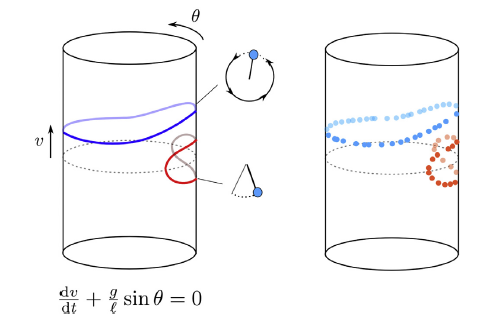
\includegraphics[width=\linewidth]{images/phase}
  \caption{Pendulum in Phase Space} % Figure caption
  \label{pendulum} 
\end{figure}

These two regimes are represented by qualitatively different trajectories in the phase space which cannot be continuously deformed into each other (in mathematical terms, they are homotopically inequivalent). By just looking at the shape of the trajectories in the phase space, we can extract information about a dynamical system. The dynamics of the simple pendulum is fully described by a differential equation depending on the length of the pendulum (l) and the acceleration of gravity (g). In more complex biological systems for example, such mathematical equations describing trajectories in the phase space are usually unknown, but current technologies allow to reconstruct trajectories from high-throughput measurements.




%\section{Association Vectors}
Relational Vectors {Winter2014}  \newline
Alpha Connnection \footcite{Amari1987}   \newline
Intuitive Combinatorial Topology 55-60   \newline
Combinatorial Topology \footcite{Hicks}   \newline
Basics of Combinatorial Topology \footcite{BasicCombinatorialTopology}   \newline
Combinatorial Topology of Groups \footcite{Everitt2009}   \newline
Combinatorics of combinatorial topology \footcite{Melikhov2012}   \newline
Torus actions, combinatorial topology and homological algebra \footcite{Panov2000}   \newline
Distributed Computing Through Combinatorial Topology - Maurice Herlihy Dmitry Kozlov Sergio Rajsbaum   \newline
A combinatorial introduction to topology - Michael Henle
Youtube on combinatorial topology \footnote{https://www.youtube.com/watch?v=DdRpkWgGf40}

\subsection{Properties}
Graph $\rightarrow$ nodes(vertices) + edges (association vectors)
\subsection{Applying to data}
\subsubsection{Examples}
\subsection{Proofs}
\subsection{Benefits of AVectors}

%\section{Self Expressision Representation}
Low-Rank Representation over the Manifold of Curves \footcite{Zhang2016} \newline
LRR Grassman Manifolds \footcite{Yin2015} \newline
Deep Subspace Clustering \footcite{Ian2017} \newline
Structural Reweight Sparse Subspace Clustering
\subsection{Data Structures}
\subsection{Constrution of A Vector}
Laws of granular solids \footcite{McElwaine2011} \newline
Discussion of a set of points in terms of their mutual distances \footnote{Young, G. and  Householder, A.S. Psychometrika (1938) 3: 19. https://doi.org/10.1007/BF02287916} \newline 
Topological vector spaces and distributions horvaths \newline
A General Coefficient of Similarity and Some of Its Properties \footcite{Gower1971} \newline
\subsubsection{Triangle law}
Youtube viddeo on Tiangle Law \footnote{https://www.youtube.com/watch?v=w8x8nETmD4w}


\subsection{Compression Advantages}
Low-Rank Representation over the Manifold of Curves \footcite{Zhang2016} \newline
LRR Grassman Manifolds \footcite{Yin2015} \newline
Deep Subspace Clustering \footcite{Ian2017} \newline
Structural Reweight Sparse Subspace Clustering
\subsubsection{Edge Bundling}
Taking relational vector for edge bundling and compression.

\subsection{Example}
Example here of compression in detail
\subsection{Special Cases}
Special Cases Section\newline
Anomaly detection

%\section{Roy Topohedron}
Isometrically compressed data from topological hypersurface to roy topohedron surface in fphase space. \newline
Prinicpal limiting nodes containing all boundary entities in a network. \newline
Surface with all i $\in$ attribute \newline
\subsection{Roy Simplex}
%1 Face of a Roy Tophedron

%\begin{figure}[H]
 % 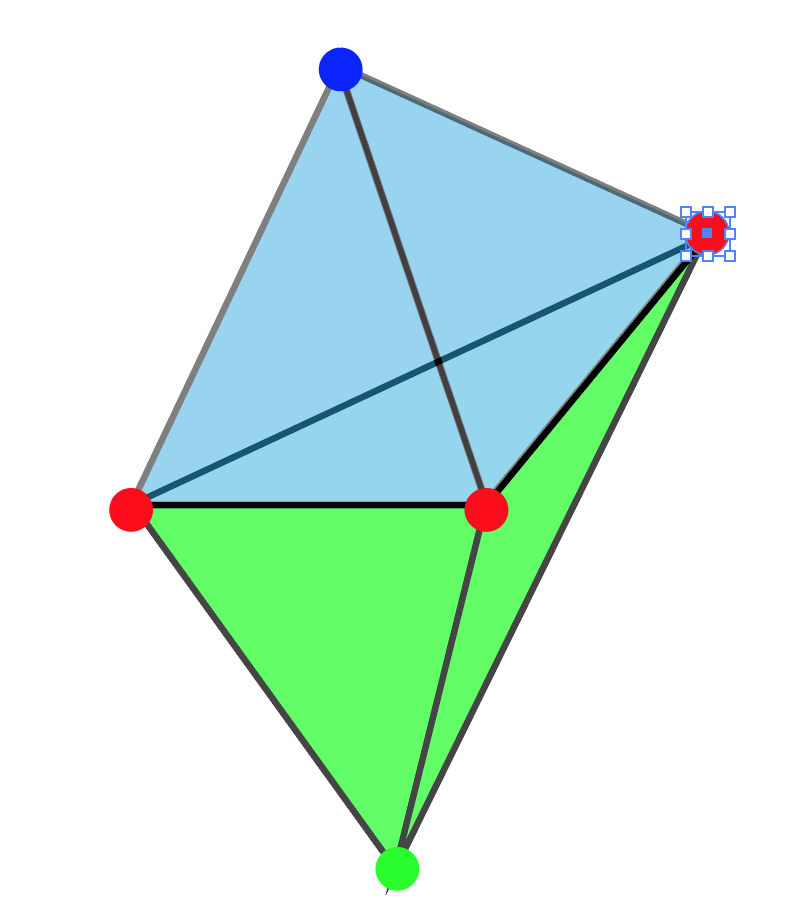
\includegraphics[width=\linewidth]{images/topohedron}
 % \caption{Roy topohedron} % Figure caption
 % \label{topohedron} 
%\end{figure}

\begin{figure}[H]
  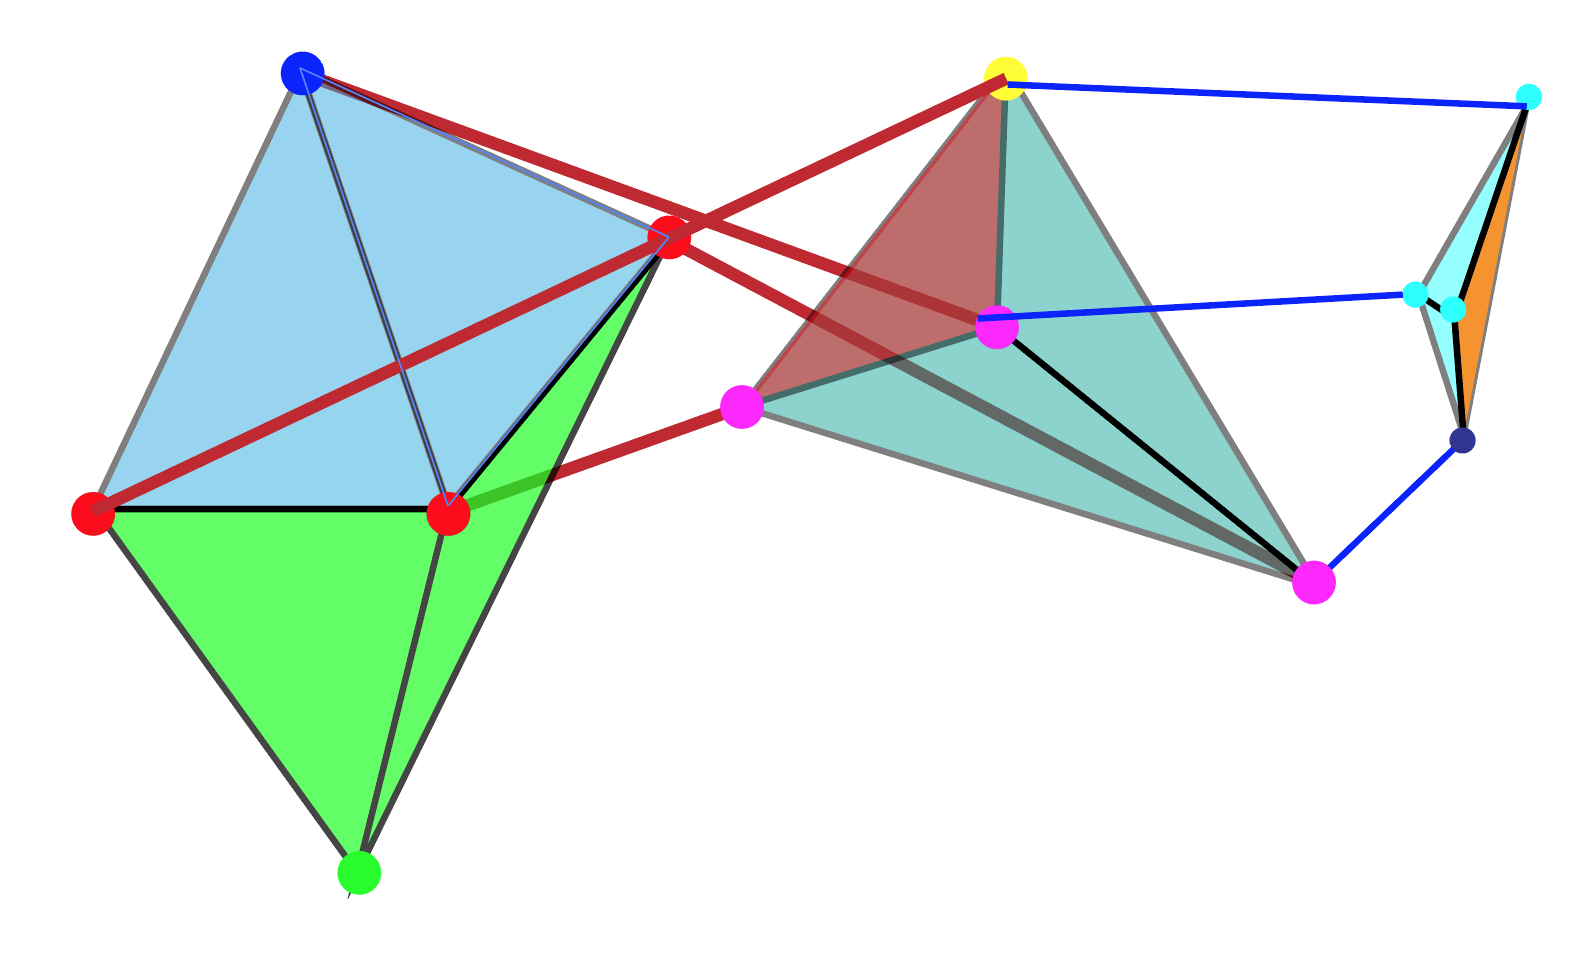
\includegraphics[width=\linewidth]{images/topoview}
  \caption{Topoview} % Figure caption
  \label{topoview} 
\end{figure}

\subsection{General Topological Properties}
Kolmogorov,Frechet,and Hausdorff space?
Seperable,
Connection properites,
Compactness Properties,
Metrizable,
Topological homogenity,
Finitely generated,
$\kappa$ resolvable
Dispersion character,
Strongly Discrete.

Simplicial Approximation Theorem
Abstract Simplical Complexes

\subsection{Topohedron Classes}


\begin{figure}[H]
  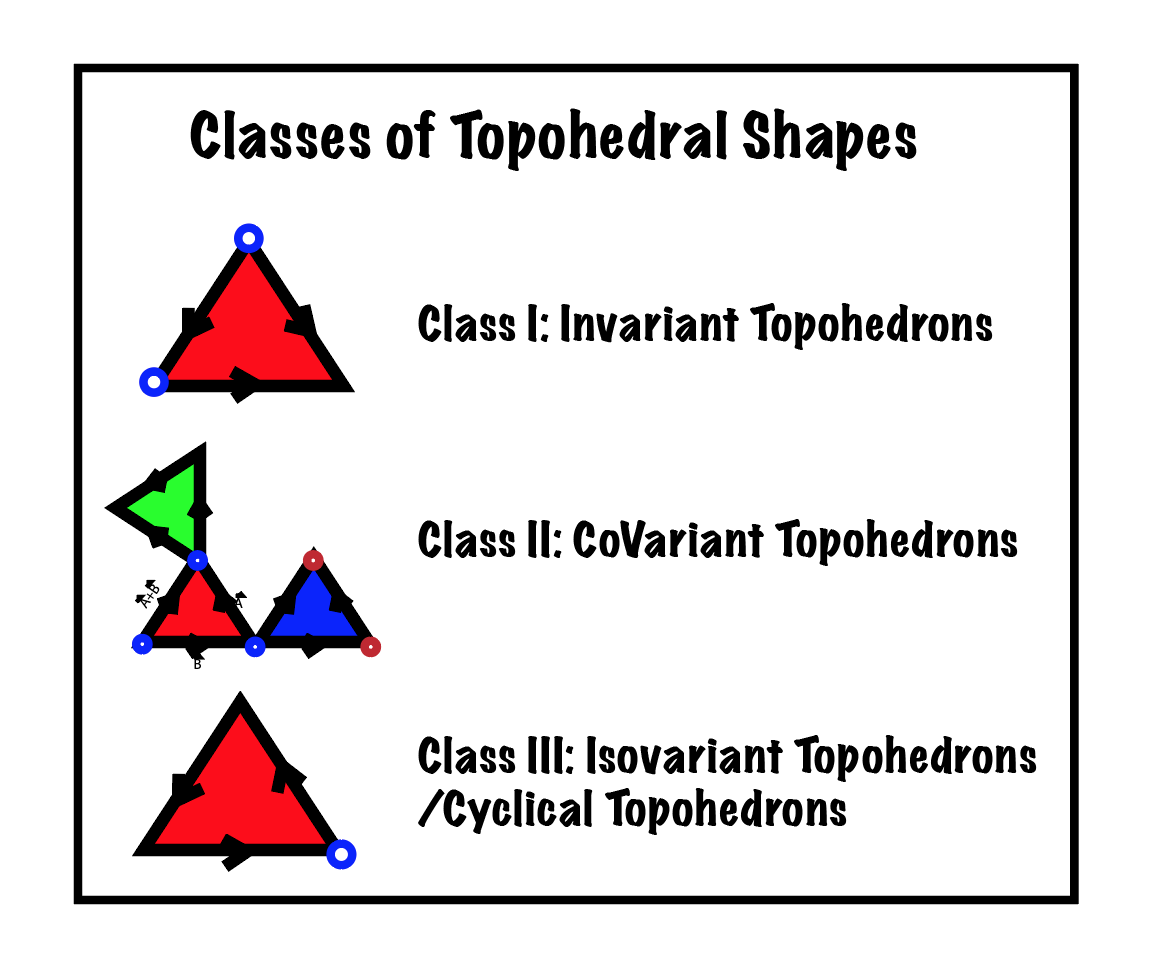
\includegraphics[width=\linewidth]{images/classes}
  \caption{Classes Explained} % Figure caption
  \label{classes} 
\end{figure}

\begin{definition}[Covariant Topohedrons]
In a covariant topohedron, at max entropy the symmetry breaks $\tau sym \in \Delta i$  \newline
Invariant under $\Delta i / \Delta S$
\end{definition}
\begin{definition}[ClassII: Invariant Topohedrons]
Invariant Topohdrons perserve symettry at $\tau sym \in \Delta i$ \newline
Covariant under $\Delta i / \Delta S$ \newline
For Both: \newline
If $\frac{W_f}{W_i} < 1 (k_i - k_f) > 0 \rightarrow class2$ \newline
If $\frac{W_f}{W_i} < 1 (k_i - k_f) < 0 \rightarrow class2$ \newline
\end{definition}


\begin{definition}[ClassIII: Isovariant Topohedrons]
Isovariant topohedrons are isolated, closed, information loops that occupy special cases of topologiacl representations.\newline
Isovariant as $\Delta i = k$
\end{definition}

\subsection{Properties}
$k_i$ is the initial size of the simplex surface\newline
$k_f$ is the final size of the simplex surface\newline
If $\frac{W_f}{W_i} \approx 1 (k_i - k_f) = 0 \rightarrow class3$\newline
If $\frac{W_f}{W_i} \ne 1 (k_i - k_f) = 0 \rightarrow class1$\newline
If $\frac{W_f}{W_i} < 1 (k_i - k_f) \ne 0 \rightarrow class2$\newline

Continutity,
Connectedness,
Convergence

\subsection{Measuring Topological Entropy}
therefore Network Entropy is defined as $\Delta S_n = \frac{\Delta K_s}{n} \times log(\frac{|W_f|}{W_i})$\newline

Check this: \footnote{https://math.uchicago.edu/~may/REU2014/REUPapers/Butt.pdf} which defined topological entropy. This also \footnote{https://www.ncbi.nlm.nih.gov/pubmed/27415290} might help, which defines the Riemannian-geometric entropy for measuring network complexity.

\subsection{Proof}
\subsection{Sample Cases}

%\section{Lens}
\subsection{Impact of Lens on Perspective}
\subsection{Homological persistence}
\subsection{Global Properties within Local Associations}


%\section{Proofs}

\section{Pipeline}
In this section we elaborate on the full algorithmic pipeline in respect to the sections as described in the previous sections. By combining isometric compression, association vectors, machine learning, phase space projections, and filters we are able to accomplish a novel approach toward data analysis which allows for two important properties: Classification and identification of stable shapes in phase space and a smooth transition between topological and graph structures. This section will demonstrate the component flow in specificsand the full pipeline. Some of the specific techniques used such as clustering, cuts, entropy measures, etc will be proposed in the following sections, however the best implementation of each pipeline component needs to be tested rigorsly and often may be application based.

See Figure 10.2 for the pipeline. 

\begin{figure*}
  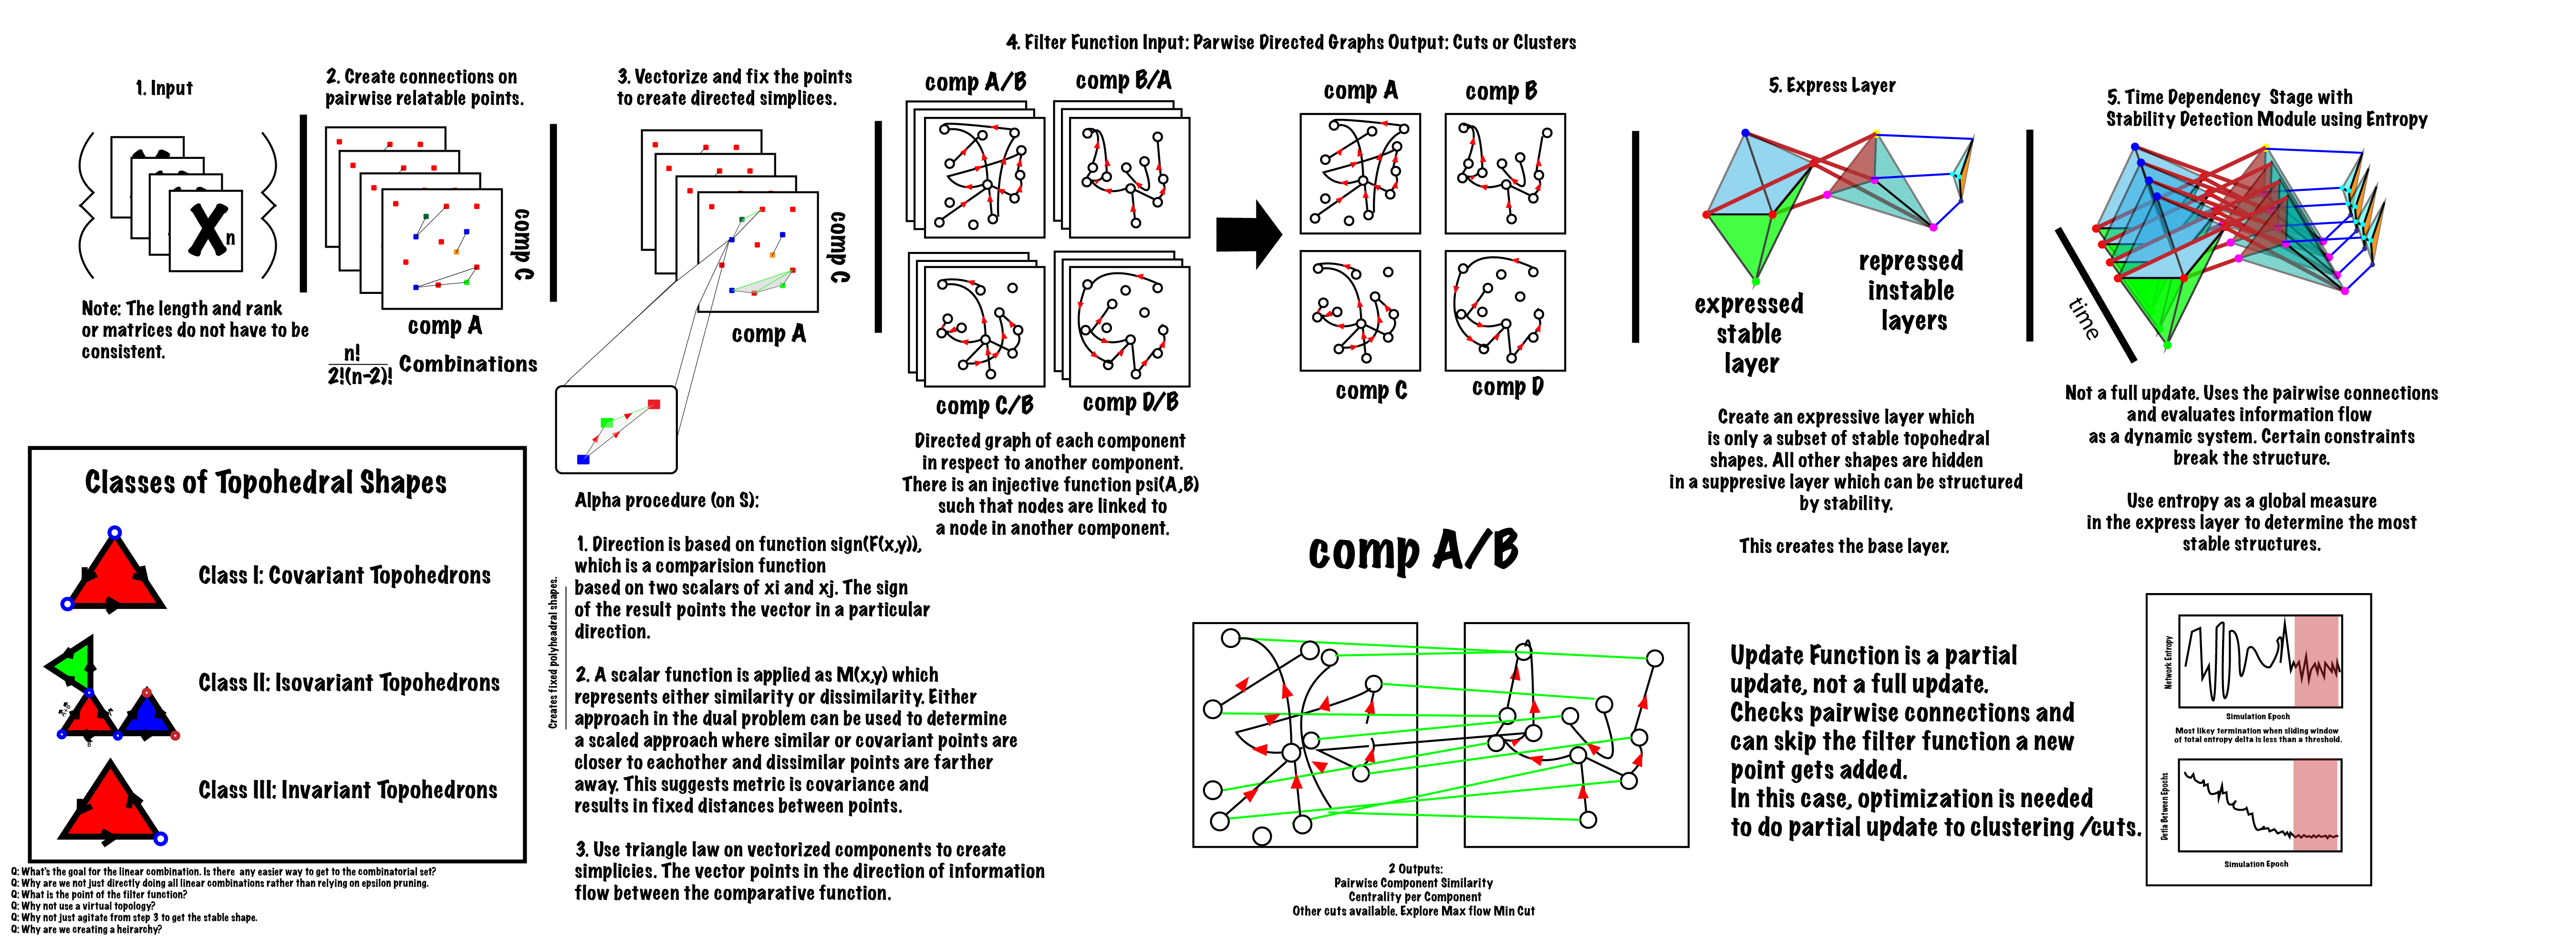
\includegraphics[width=\textwidth]{images/pipeline3}
  \caption{Pipeline}
\end{figure*}
\subsection{Step 0: Input Space}

Let $\mathbb{X}$ or the \textit{Input Space} be superset that consists of a set of $n \times m$ input matrices $X$ where $X_i = [0,N] \subseteq \mathbb{R}^d$ whose union into $\mathbb{X}$ form the toplogical set . The set of $X$ form a topological set $\tau$, due to the following properties:

\begin{itemize}
\item $X \in \tau, \emptyset \in \tau$
\item $\{O_i\}_{i \in I} \subseteq \tau \Rightarrow \bigcup_{i \in I}O_i \in \tau$ (the union of $\tau$ is in $\tau$)
\item $\{O_i\}_{i \in I}^n \subseteq \tau \Rightarrow \bigcap_{i \in I}O_{i=1}^n \in \tau$ (intersections in $\tau$ are in $\tau$)
\end{itemize}

The topological space forms a generalization of the metric space and so any metric space as an input would be sufficient to continue the problem. Due to some of our later constructions in the pipeline it is necessary that there is a bijective mapping $\psi$ for each component within $\tau$ such that $\forall \psi: x \in X \rightarrow y \in X_{y \neq x}$. Moreover, $\forall \cup_{i=0}^n x \in X$ it is one-to-one and forms $X$.   

\subsection{Step 1: Association Vectors}

From point $p \in X$ and set $S \subseteq X$ we denote the minimum distance $\epsilon$ and $\delta(p,S)$ to be the minimum distance function from $p \rightarrow S$. Similar to Vietoris–Rips complex, we evaluate all points within $\delta(p,S) \leq \epsilon$, by drawing them as connected components.

Computationally, creating the connected components is the quadratic of the points in each layer however \footcite{Piegl} there has been a variety of work done to make Vietoris–Rips approximations more computationally tractable such as Donald Sheely who achieves simplicial complexity of $O(n \log n)$ time, however we will leave future papers to discuss optimization strategies necessary for fast computation as this will require modification of traditional Vietoris–Rips constructions. 

Let us call the set connected chain $C$ whose properties include:
\begin{itemize}
\item $C \in X$ and $C \leq X$
\item $\mathbb{C} = \bigcup_{i \in I} C$ such that the union of all connected chains are the set of all connected components.
\item $\| \vec{c} \|$ denotes the length of the connected component, which is the number of edges.
\item $\| \vec{c} \| = n - 1$ where n is the connected vertices.
\item $\|\cap C_{i \in I} / \mathbb{C} \| \geq 0$ such that the intersection of all connectd chains is greater than or equal to 0. 
\item Each component in $C$ can be represented by their pairwise components such that $C_{i,j}$ represent the connection between $C_{i,j}$
\item Order invariant such that $C_{j,k} = C_{k,j}$ 
\item $\mathbb{C} = \{C_{j,k} \rightarrow C_{k,i} \rightarrow C_{i,l} \rightarrow ...\}$ such that $\mathbb{C}$ represents a connected chain which contains no disjoint components. In other words, one could trace the chain without ever having to lift his/her pencil.
\end{itemize}

To encode direction and magnitude into our pairwise connected components, we define the \textbf{Alpha Function} as stated below. 

\begin{definition} [Alpha function]
\end{definition}

Let the $\alpha$ function be an encoding function on a connected set $C$ such that $\forall(c \in C)$, there is a direction and magnitudal component such that $\forall C, (m,d \in c)$. We call each $c$ an association vector which after encoding is denoted as $\vec{c}$. Let the set $\vec{A}$ be bijective and $\vec{A} = C$ however let $C$ be a more generalized form. We call the encoding function $\alpha$, such that $\alpha(C)$ provides the necessary encodings for each vector. There are a number of consequences with this encoding, such as the fact that $\|\vec{c}\|$ is fixed and contingent to the $\alpha$ function.

In dynamic systems, these values change as the data underneath changes, thereby these values are only snapshot invariant. With perterbation to the data and time our underlying encoding undergoes state changes. As will be clear later, this is important to consider because we will use techniques to determine stable structures under pertebation and time.

\textbf{$\alpha_M$: Magnitude Function of Alpha}

Let the magnitude function be consistent with the definition of a distance function, who's length is inversely porportional to the distance encoding. Such is that larger distances are localized with further seperation and closer distances are more proximal with eachother. Let further formulization be described as below:

\begin{enumerate}
  \item $D(A_{a,b}, B_{c,d}) > 0$
  \item $D(A_{a,b}, B_{c,d})$ is finite.
  \item $D(A_{a,b}, B_{c,d})$ is ordinal with higher similarity being inversely porportional to the value.
  \item The relative encodings are scale invariant.  
\end{enumerate}  

\textbf{$\alpha_D$: Directional Function of Alpha}

Let the directional function be a singleton choice in the set $B = \{Source,Target,\emptyset\}$ where the directional component represents flow of information between source and target. For the encoding, we declare a comparitive interface $\alpha_{D}(source,target)$ which chooses an element in B which provides the directional component of the association vector. To measure information flow, we will typically use the function:  $sign(f(source,target))$ where f is a comparative function that measures information flow between the source and the target. 

  \begin{figure}[H]
  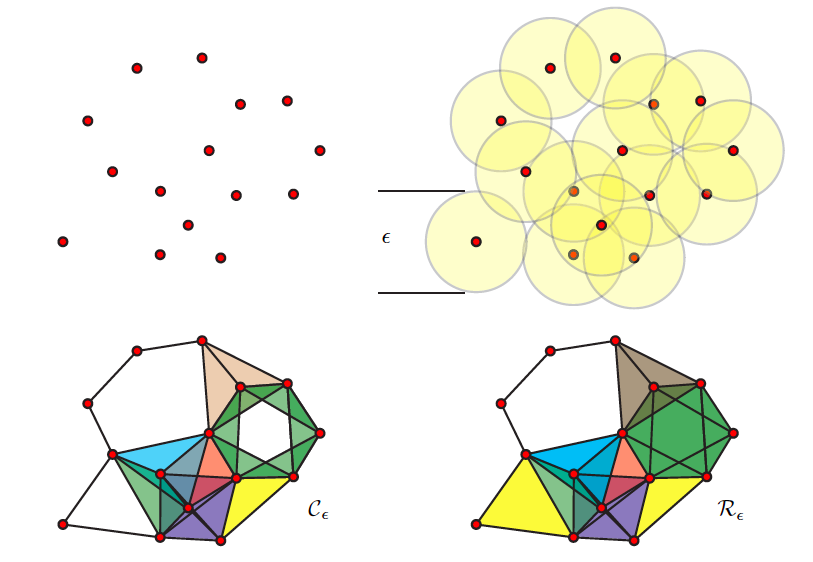
\includegraphics[width=\linewidth]{images/vrcomplex}
  \caption{A fixed set of points. Top right: Closed balls of radius $\epsilon/2$ centered at the points. Bottom left: Cech complex has the homotopy type of the $\epsilon/2$ cover. $(S^1\vee S^1\vee S^1)$ Bottom right: Vietoris-Rips complex has a different homotopy type $(S^1\vee S^2)$. Image from R. }
  \label{vrcomplex} 
\end{figure}

\subsection{Step 2: Directed Simplicial Complex}

\par Using the concept of collinearity, we can create a constrainted and directed simplex by use of the triangle law. We will term each 2-simplex as a "Roy Simplex" and the directed simplicial complex that will eventually be formed after the pipeline is finished as a "Roy Topoheadron". 

\begin{definition}[Roy Simplex]
  Let a roy simplex be a directed simplicial complex where one side is directed vector made from the collinear combination of the two other vectors that compose the 2-simplex.
\end{definition}
  Let a triangle be completable if it can be represented by a linear combination between two vectors in vectorspace. As a basis for this completion, we will use the simple vector triangle law to create collinear connected components. We represent this by equation 10 below. Using another comparative function, we look at the information flow between collinear points to provide a direction for the connecting vector. We will call this this collinear association vector, and this vector is critical for later on in the pipeline for creating stable structures.

\begin{figure}[H]
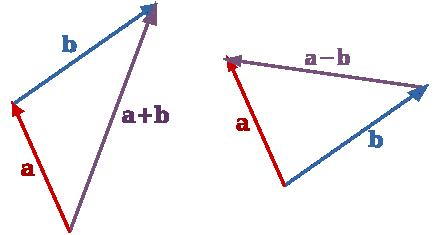
\includegraphics[width=\linewidth]{images/vectoraddition}
\caption{Vector Addition. The left is tail-head oriented vectors. To the right is coinitial vectors}
\label{vectoraddition} 
\end{figure}

\textbf{Triangle of Vector Law Addition}
\newline
If CoInitial Vectors:
\begin{equation}
      \vec{c} = \vec{a} - \vec{b} 
\end{equation}\newline
If Tail-Tail Vectors:
\begin{equation}
      \vec{c} = \vec{a} + \vec{b} 
\end{equation}
where:\\
$\vec{c}$ is the connecting vector between vectors a and b, originating at a singleton if it is coinitial.
If the vectors are tail-head oriented then $\vec{c}$ originiate from different points. 
\par We term the \textit{Dominating Vector} to be larger magnitude of two vectors |A| and |B|. To find the dominate vector is very simple. The formulate $sign(\|\vec{a}\| - \|\vec{b}\|)$ gives the dominate vector with respect to the first component. When providing direction to our generated vector, we point the vector towards the dominate vector. This is intended to mimic the flow of information from one point to another.

The generated vector we term as the \textbf{dependent vector}.

\subsubsection{Roy Simplex Classifications}

Let us denote the information state of the network as $W$ and the velocity of the information toward the beginning and end of each timestep as $W_i$ and $W_f$ respectively. Let us denote $\Delta(W)$ as the total change of information in the network through over timestep $h$ and $\partial(W)$ to be related to the component differentials of $W$.

The formation of Roy Simplicial Complexes and ostensibly Roy Polyhedrons have geometric implications that will be described below. We classify the roy simplex into three different classifications based upon the intrinsic nature of the simplex.

\textbf{[Class I] - Invariant Topohedrons:} are topohedrons that perserve symmetry under all cases. They are formed as a colinear combination of two vectors and are stable structures in the topohedron. As the flow of information changes between the dependent vector, the structure is stable and the toplogy does not change.   

\textbf{[Class II] - Covariant Topohedrons:} are topohedrons that perserve symettry however are linked simplicials on a single vertex. 

\textbf{[Class III] - Isovariant Topohedrons:} are formed by cycles in information flow and thus have no dominate vector. There are few properties unique to an isovariant topohedron. 


\begin{figure}[H]
  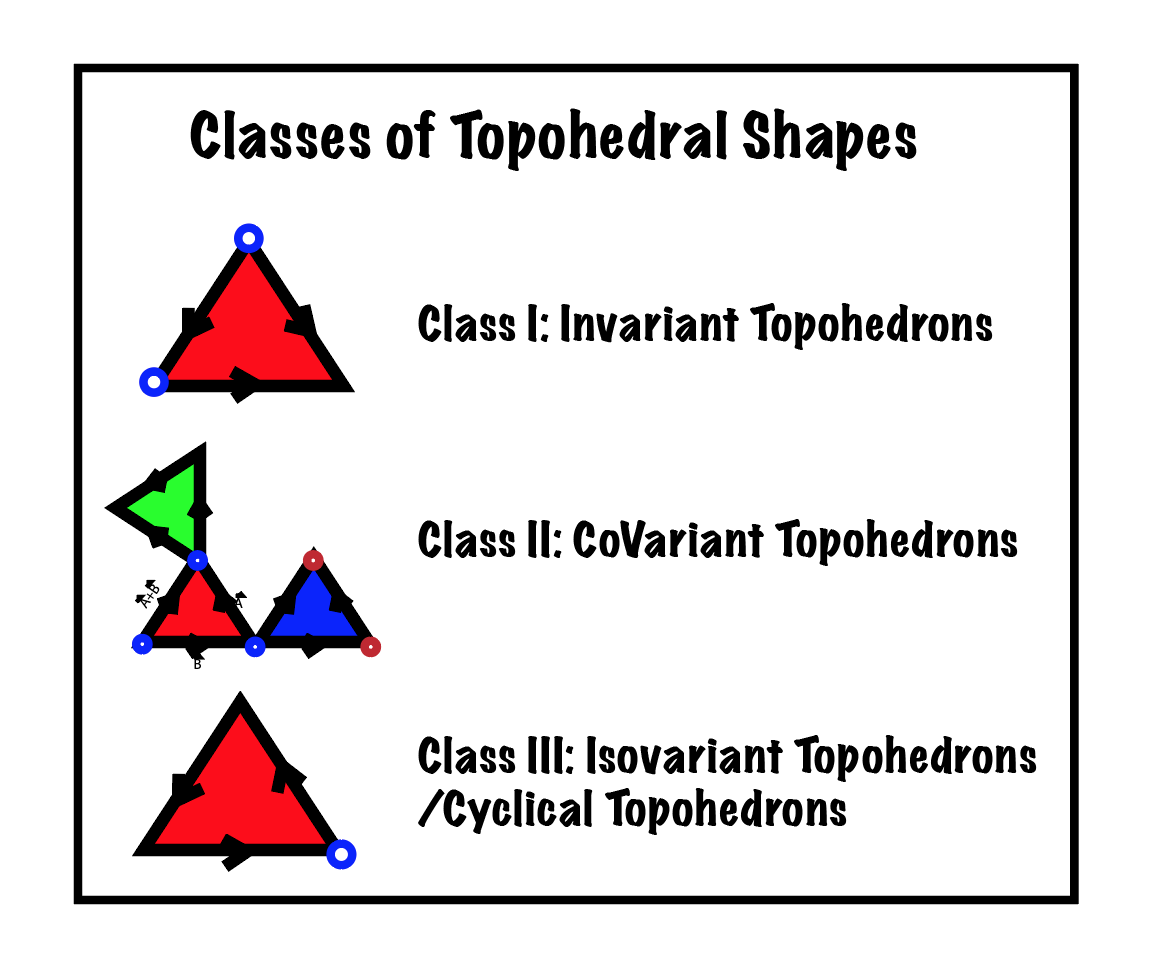
\includegraphics[width=\linewidth]{images/classes}
  \caption{Classes Explained} % Figure caption
  \label{classes} 
\end{figure}

\subsection{Express Steps}
\begin{definition}[Component Map]
  Let $\psi: A \rightarrow B$ be the component map from component A to component B which is an injective map between pairwise components. 
\end{definition}
Let us call the express step in the pipeline a lossy compression step where we isometrically compress the simplicial simplices formed in Step 3 into multi-level classifications. To do this, we employ partial clustering on filter mechanisms such as centrality and pairwise simlarity to form cardinality on the set. We use the highest rank of cardniality to form the set we call the \textit{Express Layer} and follow the expressed layer by disjoint sets called \textit{Repressed Layers}.

After filtration, three componential "Roy Simplexes" and connected to form a "Roy Topoheadron". The Roy Topoheadron has a number of special properties.

\subsection{Entropy Measurements and Stability Detection}
As a dynamic system, we can produce these "Roy Topoheadrons" over time, which allow us to monitor the development of the topology through phase space. We define the phase space of a roy topoheadron to be the shadow projection of the topological shape over time. By using a measurement of network entropy. 

Gibbs Entropy
\begin{equation}
\sigma = 1/N log \digamma
\end{equation}

where: $\digamma$ denotes the cardinality of the ensemble. Other measurements include metrics such as:\\
\newline

\begin{center}
  \textbf{Shannon Entropy}: $S = (\mathcal{L}) = - \sum_{i<j} \sum_{\alpha} \pi_{ij}(\alpha)log\pi_{ij}(\alpha) $
\end{center}
There is more work to be done to find the best entropy measurements for a dynamic system of directed topological objects and graphs. \footcite{Bianconi2009}

\subsection{Updating Topology}
Our update function does not need to recompute all steps from scratch. There are a variety of opimization steps that can be employed to increase the efficieny of update function. After the first run, we can optimize so each step updates minimalistic. The optimizations will be discussed in a seperate paper. 

\section{Discussion}
Discussion points:
\begin{enumerate}
\item Optimization strategties
\item Entropy Measures
\item Pertebation
\end{enumerate}

\subsection{Application Discussion}
\subsection{Further Work}
% \section*{Author Information Acknowledgments and Legal Declarations}
\lipsum

%\section*{Math and Code Supplements}
\lipsum


%----------------------------------------------------------------------------------------
%	BIBLIOGRAPHY
%----------------------------------------------------------------------------------------
\newpage
\newpage

\printbibliography[title={Bibliography}] 

%----------------------------------------------------------------------------------------

\end{document}
